\section{Discussion}
\label{sec:c3_discussion}

To determine the robustness of our results, and provide clues to the sources of the differences between \arepo\ and \gasoline\ simulations, we ran a number of tests varying code parameters.

\subsection{Resolution Test}
\label{ssec:c3_restest}

%low and high-resolution \arepo\ simulations experience initial mass transfer at about twice the rate of their \gasoline\ counterparts -- the accretion stream is correspondingly denser -- and experience donor disruption at approximately three orbits of the binary, rather than {\gasoline}'s four.  Two factors can contribute to this difference.  First (and based on Sec. \ref{ssec:restest}, perhaps most important), because steep density gradients near the surface of the WDs are treated differently in the two codes, and \arepo\ requires a background grid, stars relaxed in {\gasoline} tend to expand a little when transferred to {\arepo}.  Second, mass transfer in SPH can only occur by passing particles between the WDs, imposing a mass resolution limit, while in \arepo\ no such limitation exists.  This second issue exists even at the highest resolution SPH simulations performed to date, and detailed studies of the accretion stream are best done using a grid code to complement or supplement the SPH simulation \citep{guil+10, ross14}.

As noted in Sec. \ref{ssec:c3_initcond}, an \arepo\ simulation with identical mass resolution to a \gasoline\ one will have a factor of $2-3$ higher spatial resolution.  It is possible that the differences we observe between our simulations are not due to fundamental differences between the codes, but because our \gasoline\ simulation insufficiently resolves the merger.  To address this, we perform a series of \gasoline\ and \arepo\ simulations with a mass resolutions of $5\times10^{28}\,\mrm{g}$ (equivalent to $5.1\times10^4$ particles/cells and comparable to resolutions used in parameter-space sweeps by \citealt{dan+12,dan+14}), $1\times10^{28}\,\mrm{g}$ ($2.6\times10^{5}$) and $1\times10^{27}\,\mrm{g}$ ($2.6\times10^{6}$).  This factor of $50$ range in mass resolution ($\sim4$ in spatial resolution) allows us to both determine the degree to which mergers in each code change with resolution, and to compare \arepo\ runs to \gasoline\ ones at finer mass resolution.

At all four resolutions, the \gasoline\ simulations exhibit very similar behavior prior to coalescence.  The donor fully disrupts in at $\sim3.6$ orbits of the initial binary for the two higher resolution runs, while the two lower-resolution ones disrupt slightly earlier at $\sim3.2$ orbits ($\sim155-165\,\mrm{s}$).  Coalescence for the highest resolution run occurs at $\tcoal = 230\,\mrm{s}$, within $2$ seconds of the standard resolution one, while it occurs $20 - 35$ seconds earlier for the two lower resolution runs (we note the way we determine coalescence is somewhat sensitive to changes in the detailed configuration of the remnant).  Just after coalescence, all reproduce the crescent-and-void configuration, with the void being least prominent in the lowest-resolution run.  

\arepo\ also reproduces the same qualitative evolution up to coalescence at all resolutions, but donor disruption occurs within only $\sim1.9$ orbits at its lowest resolution, and in $\sim2.8$ at its second lowest.  The time of coalescence is likewise much sooner in the lowest resolution simulation, with $\tcoal = 150\,\mrm{s}$.  The highest resolution run, however, is very similar to the standard resolution one, with donor disruption occuring at $\sim3.7$ orbits ($\sim185\,\mrm{s}$) and $\tcoal$ occuring at $234\,\mrm{s}$, close to the standard run's values.  These differences are in part due to our initial conditions setup, where \gasoline\ SPH particles are directly mapped to \arepo\ cells.  WDs that are hydrostatic in \gasoline\ are not precisely so in \arepo, particularly in the poorly resolved atmosphere, and we see the WDs spuriously expanding in the first few seconds.  This effect leads to larger mass-transfer rates early in the merger, and is magnified with decreasing resolution.  Just after coalescence, all \arepo\ runs reproduce the crescent-and-void configuration except in the lowest-resolution one.

% Personal note on initial conditions: as described by Agertz et al. 2007 and Hess & Springel 2010, surface tension applies at the interface between two fluids of differing densities but the same pressure.  As particles from the less dense fluid approach the interface, they begin sampling only the density of the denser fluid (since they comprise the majority of nearby particles).  This overestimates incoming particles' densities, leading to an additional repulsive force that inhibits mixing.  I understand the qualitative picture (the SPH equation of motion uses only the density of the local particle, not its mass, so an increase in density is equivalent to an increase in mass, and this becomes a bigger and bigger problem as the particle approaches the interface, thereby reducing accelerations; these accelerations "go back to normal" as the particle moves away).  I'm unable to replicate it in equations though.  I suspect that for hydrostatic equilibrium, what's happening is that particles at the surface of the star will both have spuriously high densities and forces coming from only one side.  The latter is simply a poor estimate, but the former is a systematic offset that will shrink the size of the star and, when we map our SPH initial conditions into Arepo, create systematically high densities in the outermost layers of the star.  This means we're making a star that's missing its outer layers (because SPH doesn't have the mass resolution) and piling that material slightly deeper down in the star.  In Arepo, this would act like a spring, leading to more violent oscillations.  I'm not certain why the final state of the relaxed star in Arepo has lower central density - perhaps because the atmosphere is heated more from the oscillations, the center sees less weight?

% The lowest resolution merger in Arepo also seems to heat a bit more prior to the merger, which might be due to a combination of the hydrostatic equilibrium issue and 

\begin{figure}
\centering
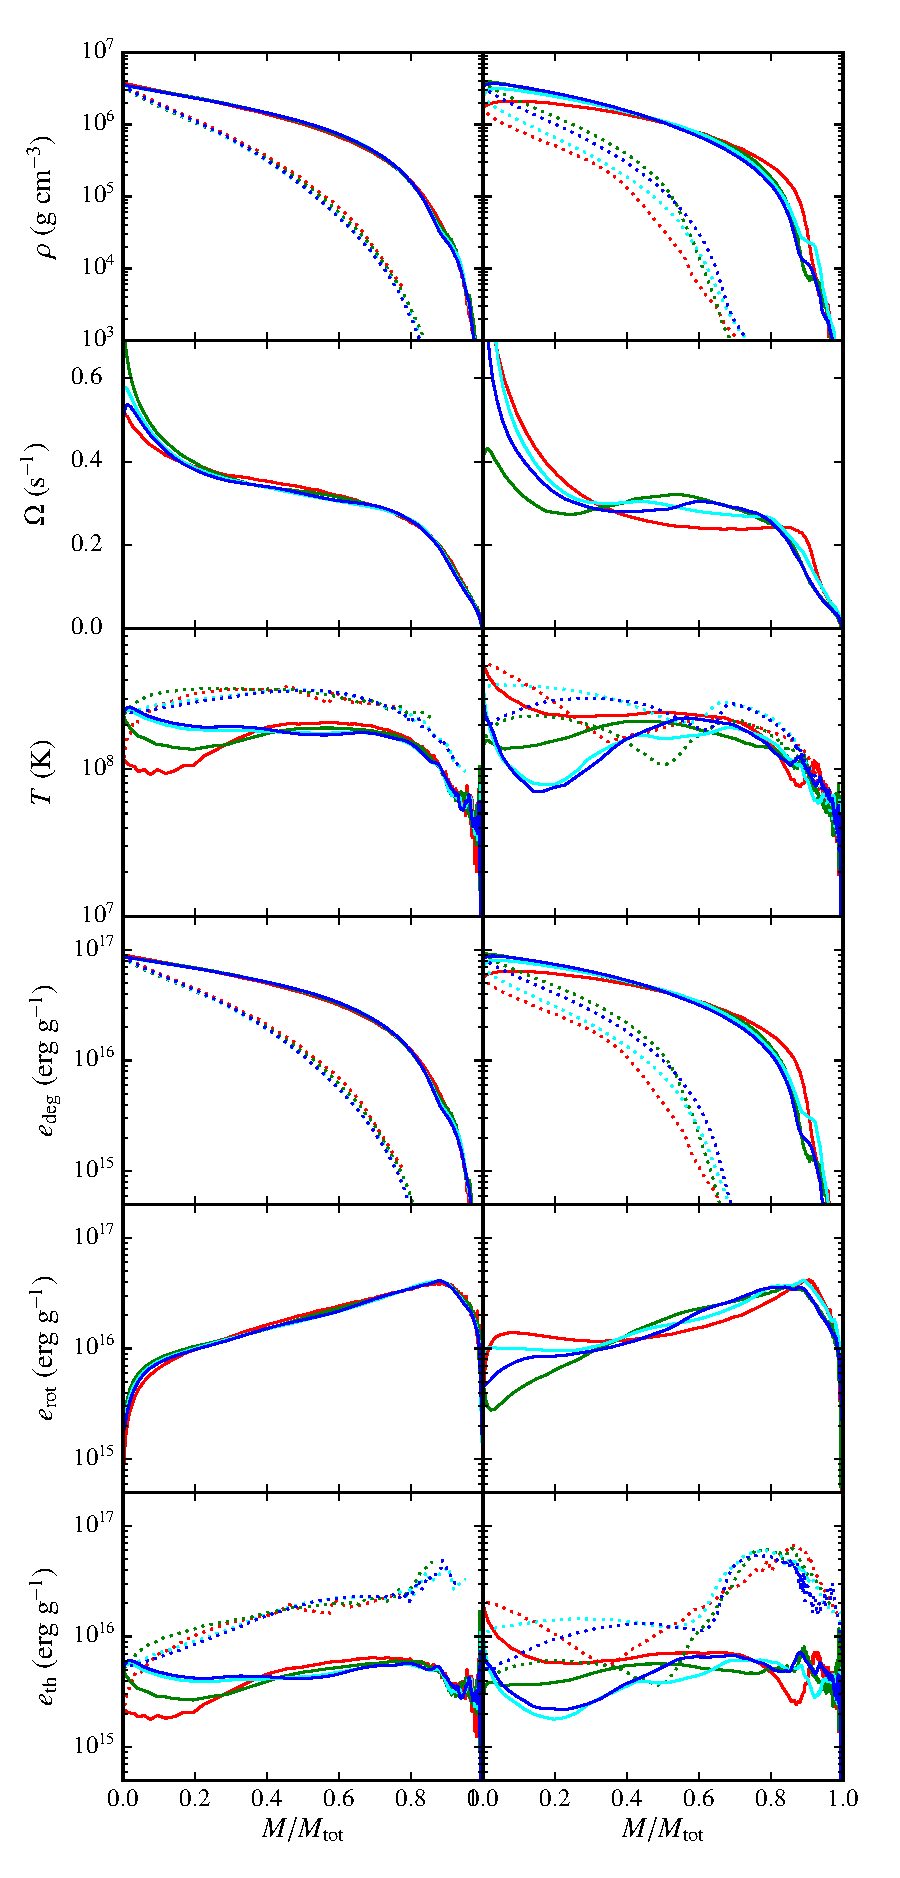
\includegraphics[angle=0,width=0.6\columnwidth]{chapter3_zhu+u/figures/curves_res.pdf}
\caption{Merger remnant profiles, as in Fig. \ref{fig:c3_curves}, for \gasoline\ (left column) and \arepo\ (right) simulations of various (initial, for \arepo) mass resolutions.  The resolutions are $5\times10^{28}\,\mrm{g}$ (equivalent to $5.1\times10^4$ particles/cells; red lines), $1\times10^{28}\,\mrm{g}$ ($2.6\times10^{5}$; green), $2\times10^{27}\,\mrm{g}$ ($1.3\times10^{6}$; cyan), and $1\times10^{27}\,\mrm{g}$ ($2.6\times10^{6}$; blue).}
\label{fig:c3_res_curves}
\end{figure}

% peak densities obtained by data mining fig:c3_res_curves (selecting the maximum equatorial density from the gas and arepo curves).

In Fig. \ref{fig:c3_res_curves}, we show the equatorial and rotational axis profiles of all simulations $99\,\mrm{s}$ after \tcoal.  The \gasoline\ remnants (left column) are all remarkably similar to one another, with the sole exception of the temperature structure at the lowest resolution.  The disk and core-envelope masses as well as the partitioning of internal energy are all within $3$\% of their values at the standard resolution reported in Sec. \ref{sec:c3_results}.  The central densities of the remnants also deviate by $\lesssim5$\% from their mean value of $3.6\times10^{6}\,\gcc$.  The \arepo\ remnants (right column) are less uniform: masses and energies vary by $\sim5-10$\% from those in Sec. \ref{sec:c3_results} for all except the lowest resolution run, which has $\sim50$\% more total thermal energy and a $\sim25$\% less massive disk.  The maximum density ranges from $3-4\times10^6\,\gcc$ for all resolutions except the lowest one, where it is $\sim2\times10^6\,\gcc$.  The variations between \arepo\ curves in Fig. \ref{fig:c3_res_curves} reflect variations in their crescent and void.  While at the highest two resolutions the crescent is clearly colder, with a temperature of $\sim5\times10^7\,\mrm{K}$, in the second lowest resolution run its temperature is $\sim1\times10^8\,\mrm{K}$, and in the lowest resolution one the remnant core never forms a crescent at all, instead appearing as a dumbbell-shaped object that transforms into a spherically symmetric one within $\sim500\,\mrm{s}$ of coalescence.  During this time, global angular momentum decreases by $\sim12$\% (Fig. \ref{fig:c3_fix_angmo_nar}), and a $<10^7\,\mrm{K}$ ring of material spuriously forms at the interface between donor and accretor, both indicating that this run is too poorly resolved to simulate the merger.  At all other resolutions, however, the crescent and void survive until the end of the simulation at $1000\,\mrm{s}$.

The crescent-void configuration also appears, but then fades away over several hundred seconds, in all \gasoline\ simulations.  To check if the longevity of the configuration is resolution-dependent, we turn to a measurement of non-axisymmetry -- introduced in Sec. \ref{ssec:c2_mergercomplete} -- using $|f_i|/|f_0|$, the ratio of largest non-zero to zeroth Fourier coefficient of particles or cells binned in azimuth.  For all simulations, the largest non-zero Fourier coefficient is the first, and the time when the hot void disappears roughly matches the time when $|f_1|/|f_0| = 0.01$, which we call $t_f$.  We find, from lowest to highest resolution, $t_f = 426\,\mrm{s}$, $483\,\mrm{s}$, $515\,\mrm{s}$ and $513\,\mrm{s}$, which suggests $t_f$ is resolution dependent, but converges at $t_f \approx 500\,\mrm{s}$.   All \arepo\ simulations maintain $|f_1|/|f_0| \gtrsim 0.1$ for $\gtrsim 1000\,\mrm{s}$, except for the lowest-resolution run, which drops to $|f_1|/|f_0| \approx 0.02$ by the end of the simulation.

%-- roughly corroborated by visual inspection of the remnant's non-axisymmetry --

We thus conclude that the largest difference between the \gasoline\ and \arepo\ simulations -- the survival of the crescent-void configuration long after the merger -- is the case for all resolutions.  The void persists for hundreds of seconds in all but the lowest-resolution \arepo\ simulation, while even in the highest-resolution \gasoline\ one it smears away, disappearing within $\sim 250$ s after coalescence.  This is evidence that spatial resolution alone is insufficient to explain the diverging behavior of the codes.  We also find that \gasoline's results change little between all resolutions, while \arepo's results only appear to agree at higher ones.  This bodes well for merger parameter-space studies using low-resolution SPH simulations (eg. Ch. \ref{ch:ch2}, \citealt{dan+14}; the latter finds similar results in their resolution study unless nuclear burning becomes important during the merger), but an equivalent study in \arepo\ would require a mass resolution finer than $\sim1\times10^{28}\,\mrm{g}$ (and ideally closer to our standard resolution of $2\times10^{27}\,\mrm{g}$) to guarantee qualitative accuracy with higher-resolution runs.

\subsection{Varying Viscosity in \gasoline}
\label{ssec:c3_vary_visc}

Artificial viscosity, which is essential in SPH for proper shock capture, has been a major issue for white dwarf merger simulations for decades (eg. \citealt{guerig04, loreig09}) because it spuriously shears differential rotation into rigid rotation, dumping excess energy into heat.  This viscosity cannot simply be mitigated by resolution, and we cannot run our mergers with zero artifical viscosity without neglecting shock heating and introducing unphysical particle behavior (Sec. \ref{ssec:c3_sph}).  We can, however, increase and reduce its strength to see what effect it has on our simulation results, as in Sec. \ref{ssec:c2_viscprescrip}.

We ran \gasoline\ simulations of our merger with a mass resolution of $1\times10^{28}\,\mrm{g}$ and artificial viscosity with fixed coefficients of either $\alpha\,=0.05$, $\beta\,=0.1$, or $\alpha\,=1$, $\beta\,=2$ (the Balsara switch is still active), comparing them to the variable-viscosity run at the same resolution in Sec. \ref{ssec:c3_restest}.  The low-viscosity simulation experiences donor disruption at $\sim3.1$ binary orbits, and coalescence at $\tcoal = 206\,\mrm{s}$, while the high-viscosity one experiences disruption at $\sim3.4$ orbits and coalescence at $220\,\mrm{s}$, values that are quite similar to those of the variable-viscosity run.  This similarity is to be expected, since mass transfer and donor disruption are governed by tidal forces, which are unchanged between the simulations.  During coalescence, the evolution of the variable and high-viscosity runs is similar.  In the low-viscosity run, however, the donor's accretion stream produces a contiguous hot ring around the accretor during coalescence, rather than the string of vortices seen in row 2 of Fig. \ref{fig:c3_diagslice}, and perturbes the accretor far less.  As a result, no distinct void ever forms, though the remnant core is distorted into a bean shape.  Within $\sim25\,\mrm{s}$ of coalescence, the void in the high-viscosity simulation is already fast-disappearing, having a radius less than half that of the variable-viscosity run.  $t_f = 358\,\mrm{s}$ and $487\,\mrm{s}$ for the high and low-viscosity runs, respectively, compared to $483\,\mrm{s}$ for the variable one.  The similarity of the latter two values is likely because the variable-viscosity run tends toward the same $\alpha$ and $\beta$ values as the low-viscosity one in the absence of shocks (though it may also partly be coincidence, since the low-viscosity remnant does not have a hot void to begin with).  At $\sim500\,\mrm{s}$, the remnant has become axisymmetric in all three codes, but in the high-viscosity run the interior $\sim0.8\,\Msun$ of the remnant is also rigidly rotating with $\Omega = 0.33\,\mrm{s}^{-1}$.

%and features a nearly uniform temperature of $2 - 2.5\times10^8\,\mrm{K}$. 

As expected, then, the high-viscosity simulation rapidly spins down to axisymmetry while eliminating differential rotation, showing that excess artificial viscosity contributes to the disappearance of the crescent-void configuration.  The low-viscosity simulation, on the other hand, primarily shows the importance of increasing $\alpha$ and $\beta$ during coalescence in order to properly capture shocks and shearing interactions between donor and accretor.

% Void sizes use the DENSITY intensity maps, not temperature.

\subsection{Sources of Differences Between Simulations}
\label{ssec:c3_differences_merger_process}

What explains the differences between simulations in \gasoline\ and \arepo, and, critically, which is more physically accurate?  This question boils down to whether or not the crescent-and-void configuration should be long-lived, as seen in \arepo, or should disappear over several hundred seconds as the remnant becomes axisymmetric, as seen in \gasoline.

% At this point I'm not entirely sure if the one-armed spirals seen in other simulations are tidal ``fallback'' tails or the m = 1 instabilities that we see...(see dan+11 and dan+14 and search for "spiral")

Instabilities generating persistent $m = 1$ spiral waves that carry away angular momentum are common features of astrophysical disks, and have been studied, for example, in the contexts of star formation \citep{adamrs89, shu+90, lin15, kratl16} and supermassive black hole accretion \citep{hopkq10}.  They have also been seen in WD merger remnants: \cite{kash+15} map the remnant immediately after coalescence from an SPH-based (highly super-\Mch) $1.0-1.1\,\Msun$ CO WD merger simulation into \flash.  They find that the merger remnant core, though not crescent-shaped, drifts off of the center of rotation and drives an $m = 1$ spiral perturbation in the disk around it for $\sim100\,\mrm{s}$.  They argue this is a variant of the ``ARS instability'' \citep{adamrs89, shu+90}, where non-axisymmetric perturbations acting on a star surrounded by a marginally Toomre-stable ($Q \lesssim 3$ at corotation) Keplerian disk move the star off the system's center of mass while generating a spiral wave in the disk.

Meanwhile, recent Eulerian simulations of binary neutron star mergers \citep{pasc+15, radibo16} see the formation of a crescent-and-void configuration with corresponding $m = 1$ spiral instabilities.  \cite{pasc+15} attributes the formation of their spiral wave to a dynamic instability found by \cite{cent+01} and \cite{saijbs03} to occur in axisymmetric equilibrium polytropes with toroidal density structures, a ratio of kinetic to potential energy $T/|W| \gtrsim 0.14$, a relatively soft $n \lesssim 2$ polytropic EOS, and high differential rotation \citep{saijbs03}.  A similar phenomenon was observed by \cite{ott+05} in their post-bounce core-collapse supernova core of $T/|W| \approx 0.08$.  \cite{wattaj05} and \cite{muhl+14} suggest this ``low $T/|W|$ instability'' may be a corotational shear instability, related to the \cite{papap84} instability for thick accretion torii.

% The cent+11 doesn't last forever - once the spiral destroys the crescent, it dies away (Saijo+03)

The conditions within our remnant are somewhat different those above.  Unlike the ARS setup, our inner disk is thick (scale height and disk radius are within an order of magnitude of each other) and has a Toomre parameter of $Q \approx c_s\Omega/\pi G \Sigma \gtrsim 8$ for $\varpi \geq 1\times10^9\,\mrm{cm}$ ($\Sigma$ is the disk surface density), somewhat too high for the ARS instabilty to act.  While the remnant core has a $T/|W| \approx 0.11$ following coalescence and is roughly toroidal in shape, it is already heavily perturbed and the spiral mode already visible once the transient features from the merger itself dissipate, making it difficult to identify a period of growth for the instability.  The behavior of our \arepo\ merger remnant may represent some combination of these instabilities, or possibly a novel, but related, phenomenon.  Further analysis is needed, but for now the existence of other $m = 1$ instabilities that drive angular momentum transport lends support to the physical validity of our results.

%this is a factor of a few higher than those in \citealt{kash+15}

% Values at the base of spiral wave eyeballed from density and temperature plots at t = 500 s in Arepo High Res 

Note that in \cite{kash+15}, the spiral wave drives an inflow of material into the dense remnant core, heating a region of the core at $\sim7\times10^6\,\gcc$ to $\gtrsim3\times10^9\,\mrm{K}$; this region detonates $109\,\mrm{s}$ into the simulation, destroying the remnant.  We also observe heating at the base of the spiral wave in our sub-\Mch\ remnant, but this region ($\rho \approx 9\times10^5\,\gcc$) only reaches $\sim3\times10^8\,\mrm{K}$, well below the $\sim6\times10^8\,\mrm{K}$ needed for carbon ignition.

At the time of this writing, we have not yet been able to conclusively pinpoint the features in \gasoline\ that cause its simulations to differ from \arepo's.  Nevertheless, we discuss below a few hints that may point the way forward.  It should first be said that gravitational instability in protoplanetary disks have long been successfully simulated in SPH \citep{ricela05, merub10, rogew12}, and for the $\sim200\,\mrm{s}$ that the remnant core is visibly non-axisymmetric, an $m = 1$ spiral mode is also visible.  This leads us to suspect that the difference resides in how the crescent is evolved in SPH (though we leave open the possibility that the smearing out of the wavefront due to poor resolution in the disk is also a contributing factor).  

The high-viscosity run in Sec. \ref{ssec:c3_vary_visc} suggests artificial viscosity may play a role in prematurely smearing out the crescent even when $\alpha$ and $\beta$ are being dynamically controlled.  Our MHD merger performed in \arepo\ (Ch. \ref{ch:ch4}) is influenced by magnetic viscosity following coalescence, and also shows the crescent becoming axisymmetric within several hundred seconds.  Another possible culprit is the surface tension that results from poor discontinuity treatment in traditional SPH, which \cite{hesss10} shows can lead to an overdense ellipse at pressure equilibrium with its underdense surroundings spuriously deforming into a sphere.  While the boundary between the crescent and void is not as sharp a discontinuity, the temperature and density do change by a factor of $3$ over a single smoothing length, and so may be influenced by this effect.  We can test if this is the case by performing the same SPH merger using \textsc{Gasoline2}, which has improved entropy mixing and pressure-averaging across discontinuities.

%\cite{dval+06} performed an extensive battery of tests on 17 independent codes, 15 Eulerian and 2 SPH, simulating in two dimensions a planet on a circular orbit interacting with a protoplanetary disk.  The planet is expected to tidally excite a spiral wave from each of its two Lindblad resonances and open a density gap in the disk.  The Eulerian codes all reproduced these broad features as well as a number of non-linear ones such as vorticies at the, and their azimuthal and radial density profiles broadly agreed in shape - in many cases they numerically agree to within a few percent \textbf{check with pavel?}.  The SPH codes, on the other hand, produce gaps with poorly resolved boundaries (or in the case of shallow gaps, a poorly resolved gap in its entirety) and highly diminished spiral waves.  SPH density density profile had both different shapes and substantial systematic offsets.  Consequently, the tidal torques between the sprial waves and the planet measured by the Eulerian codes was far stronger than the torques measured by the SPH codes.  \cite{dval+06} speculated these differences were due to the diffusive nature of SPH, as well as code features like the Balsara switch designed to reduce viscosity in shear flows also leading to poor shock capture in those same regions.

%Artificial viscosity has long been cited as hindering the formation of spiral shocks under conditions theoretically favourable to their production (ex. \citealt{yukabm97, lanzb97, lanz03}).  In particular, sprial waves more readily develop in 2D disk simulations than in 3D due to the reduced effect of artificial viscosity in 2D \citep{lanz03}.  \cite{lanz10} attempts a more physically realistic implementations of artificial viscosity, and find stronger spiral waves develop in accretion disks as a result.

%%\lanza 10 a attempt to mitigate artificial viscosity by, and \lanza 10 replaced artificial viscosity in the SPH momentum and energy equations with an equation of state that captures the increase in pressure due to physical dissipation.  Tests using these modifications show much stronger accretion disk spiral waves than equivalent standard SPH simulations.

%%COMMENT: The papers cited above are annoyingly hard to read.  In lanza 10 b, the general implementation of the EOS results in an accretion ring rather than a disk.  Lanzafame cites this as being because physical dissipation is necessary for maintaining an accretion disk.

%-In early stages, artificial viscosity in Gasoline greatly increase core heating \textbf{reanalyze low and high viscosity SPH runs}
%-\textbf{Check that T/|W| is not applicable by looking at FLASH100}
%-

%\begin{figure*}
%\centering
%\includegraphics[angle=0,width=1.0\columnwidth]{temp.pdf}
%\caption{T/|W| (instability criterion).  Bar amplitudes (Fourier moments)?}
%\label{fig:toverw}
%\end{figure*}

%Spiral waves has long been cited as an alternative to magneto-rotational instability for transporting angular momentum in accretion disks (\citealt{}, \citealt{balb03} and references therein), in particular to accrete material from a disk onto a white dwarf (eg. \citealt{}) and facilitate the inward migration of terrestrial planets (eg. \citealt{kleyn12}). 
